\section{議論}

\subsection{『わかるらんど』の思想}

近年、学会などでタイムライン表示のテキストチャットが
利用される機会が増えている\cite{WISSのチャットの報告論文}。
学会チャットシステムを利用すると、
発表中に参加者が意見交換したり疑問を表明したりできるといった利点があるが、
以下のような問題も存在する。

\begin{itemize}
\item 多数の人間が同時に投稿すると投稿内容がすぐに見えなくなってしまう
\item 投稿の多いアクティブな人ばかりが目立ってしまい、消極的な参加者は議論に参加しにくい
\end{itemize}

一般に、会議などで特定の人だけが沢山発言するのはよくあることであるが、
誰もが気軽に意見を表明できる環境を構築できれば有意義であろう。

「On Air Forum」は、日本ソフトウェア科学会主催のWISSで利用されている
コミュニケーションシステムである。
「On Air Forum」のWISS2009の実証実験\cite{nishida2011}では、
全参加者の半分弱しかログインして1回以上発言していない.
WISS2015では、252アカウントが1回以上発言し総発言数は2,948回であったが、
発言数上位20\%の50アカウントによる発言が総発言数の78.1\%にあたる2,305回を占めていた(図\ref{wisschat})。
また、発言数が10回未満のアカウントは190アカウントで、これは全アカウントの75.3\%にあたる。

\begin{figure}[h]
\centering
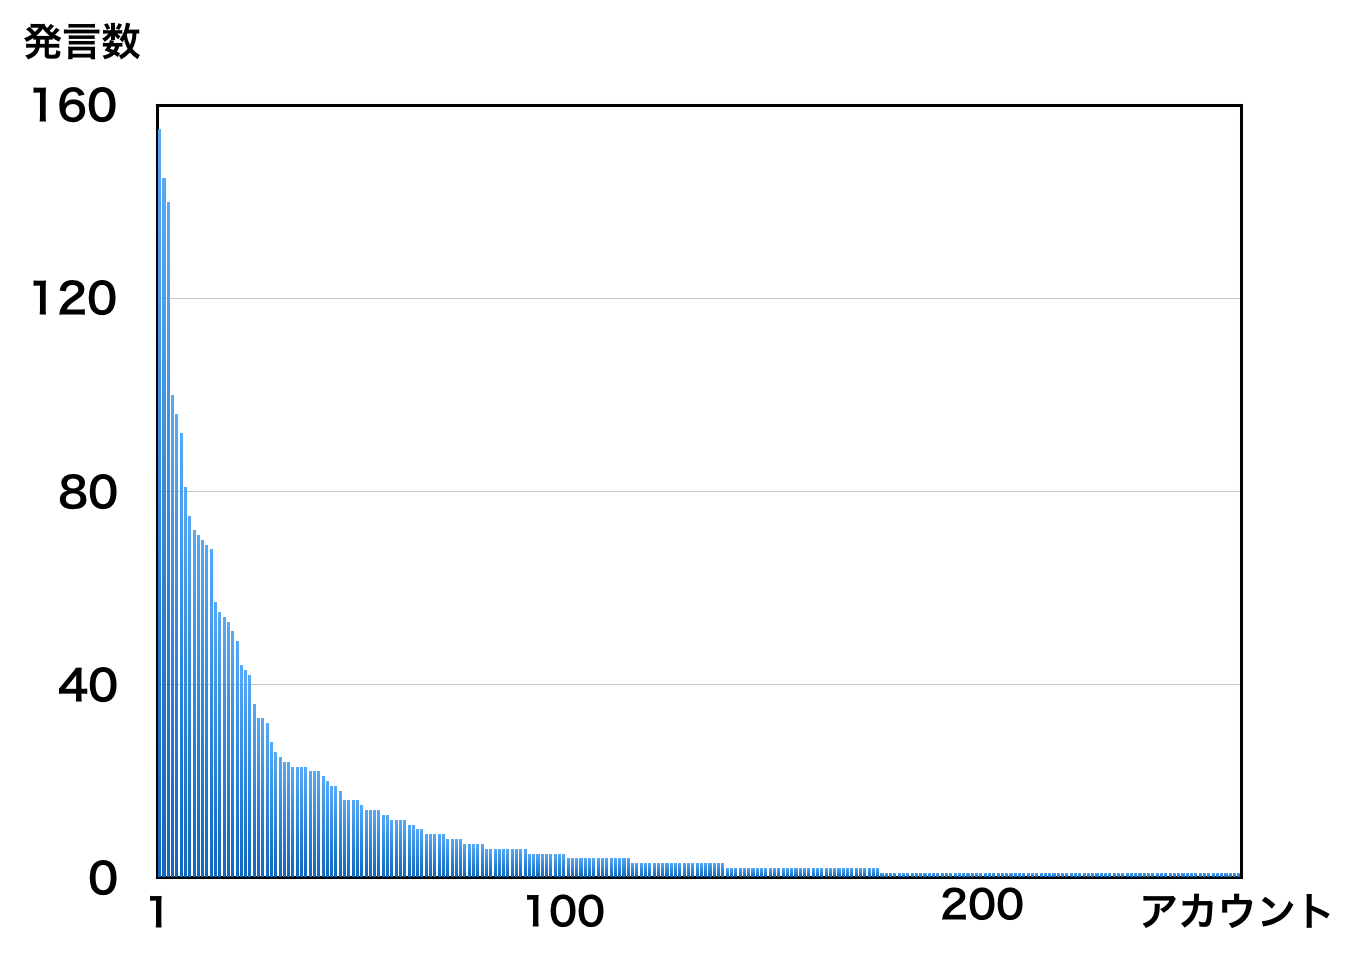
\includegraphics[width=7cm]{images/wisschat.png}
\caption{WISS2016のチャットにおけるアカウント毎の発言数}
\label{wisschat}
\end{figure}

『わかるらんど』はユーザの表示領域が均等に決まっているため、
タイムライン表示のように投稿数が多い人ばかりが目立つということがない。
また、長いテキストを入力すると表示される文字が小さくなるので、
150人程度で利用すると長い文字は小さすぎて読めない。
必然的にユーザは図\ref{wakaruland150}のように短文を入力することを強いられる。
『わかるらんど』では長文の高度な発言は期待しておらず、
「なるほど」「わからん」「笑」などといった相槌のようなものを
視覚化してひと目で把握できるようになることを期待している。
学生、先生、企業に所属する人等様々なバックグラウンドの人が入り混じった状況で
「下手な発言ができない」「気の利いたことを言わなければならない」という
投稿を躊躇させる要素を限りなく減らし、
本当は議論に参加したいけど声が出ない/手を上げる勇気がない人でも
「なるほど」「わかる」などを『わかるらんど』に投稿することで「参加」することができる。
テキストで記述すると長くなってしまう内容も
画像スタンプを投稿することで分かってもらうことができると考える。
また、長いテキストを投稿するには適していないので『わかるらんど』を使って議論することは難しいが、
多くの会議やコンファレンスでは発表後に議論の時間が設けられているため議論はその時に行えばよい。

\begin{figure}[h]
\centering
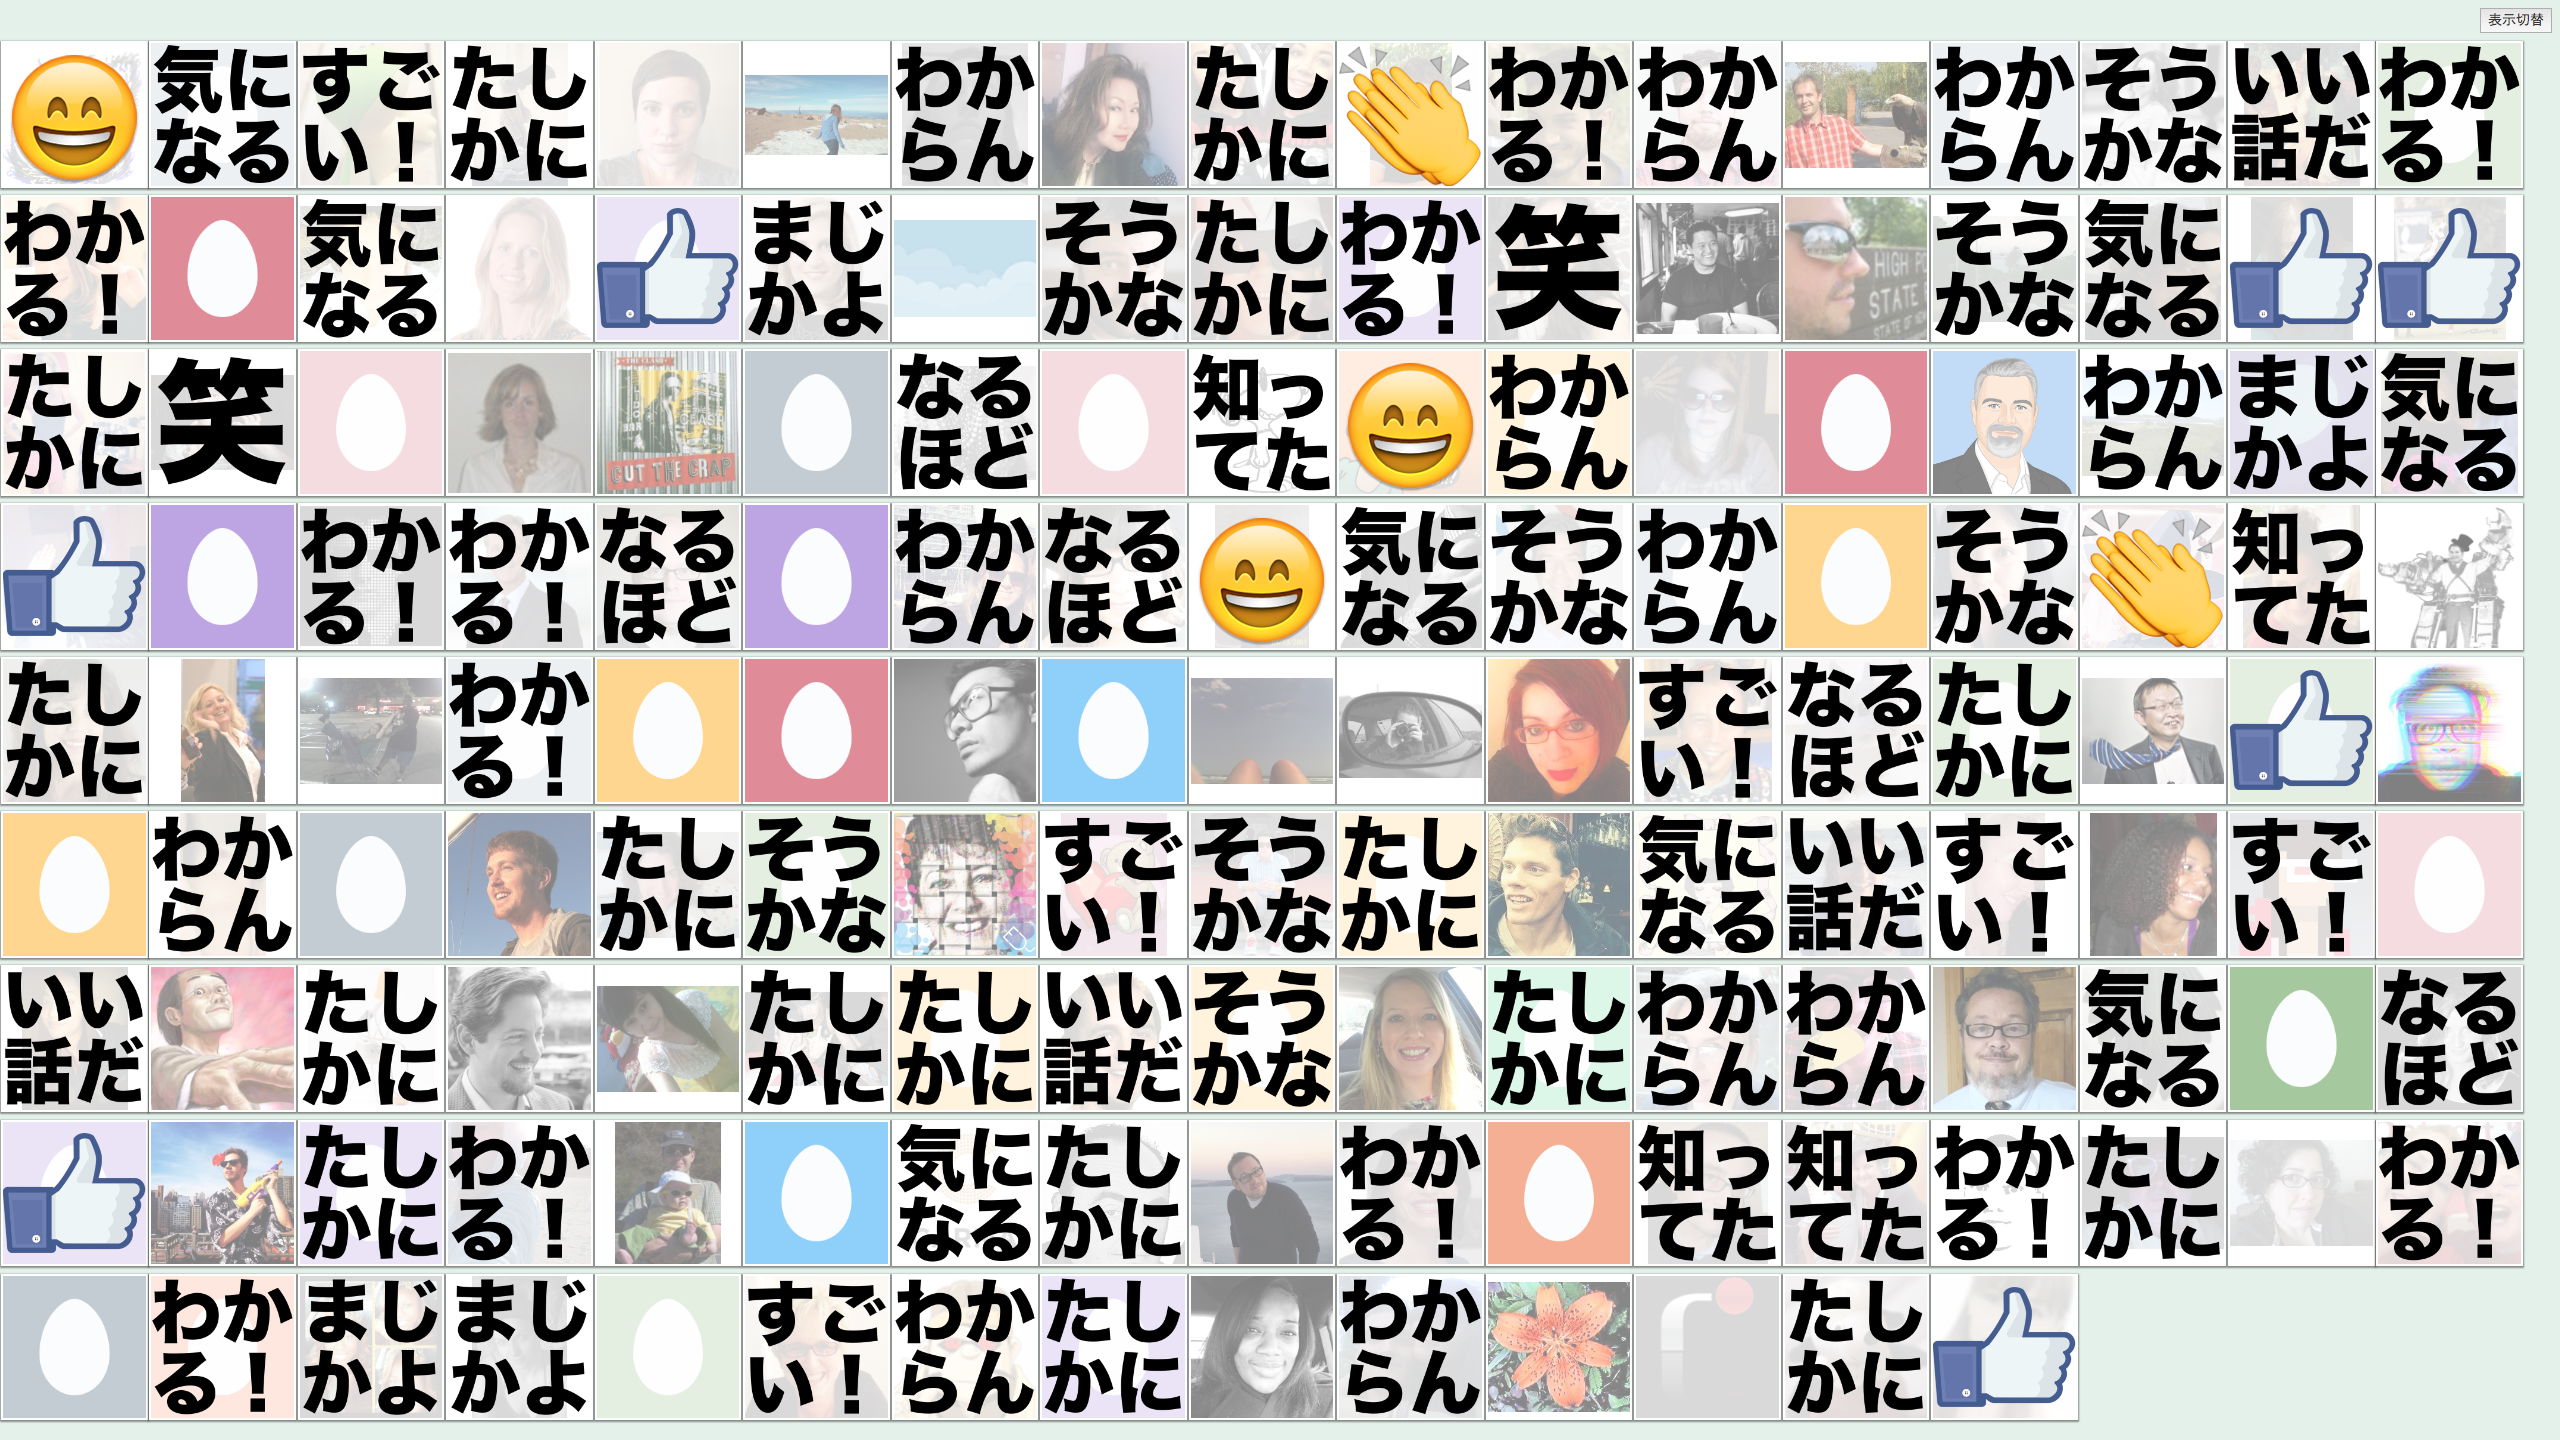
\includegraphics[width=8cm]{images/wakaruland150.png}
\caption{150人で『わかるらんど』を使用したイメージ}
\label{wakaruland150}
\end{figure}

\subsection{研究室においての利用経験}
我々の研究室では、研究室内のディスプレイに研究室メンバー全員のリアクションと
部屋の明るさ、温度、最後に研究室のドアが開いた時間を表示した『わかるらんど』を
常に表示して、約6ヶ月の間利用してきた。
ミーティングの時間には積極的に『わかるらんど』を利用した。
普段発言の少ない人でも何らかの反応を表明したり、
誰かが面白いことを言ったときに「笑」というリアクションが並ぶと面白かった。
また発表者としても、聴衆が自分の発表を聞いてくれているかどうかわからないときに
『わかるらんど』にリアクションを投稿してもらうことで、聴衆がみんなPCの画面を見ていても
何らかの投稿があれば話を聞いているということがわかるようになった。
自分が研究室にいないときでもリアクションを投稿して、
研究室でも自宅でも研究室メンバーの気分や研究室のセンサ情報が見られるようになった。

研究室で利用しているチャットでチャットボットに話しかけることで、研究室の
\begin{itemize}
  \item ドアの鍵を開ける
  \item 照明を点ける/消す
  \item 明るさを知る
  \item 気温を知る
\end{itemize}
ことができるが、『わかるらんど』と組み合わせることで非常に便利に使うことができた。


